\begin{enumerate}
\item Which of the following graphs are trees?
\begin{center}
\begin{tabular}{c c c c}
\begin{tikzpicture}
  \GraphInit[vstyle=simple]
  \tikzset{VertexStyle/.append style={scale=0.3}}
  \SetGraphUnit{1.4}
  \Vertex{a}
  \EA(a){b}
  \EA(b){c}
  \SO(a){d}
  \EA(d){e}
  \EA(e){f}
  
  \Edge(a)(d)
  \Edge(d)(b)
  \Edge(b)(e)
  \Edge(e)(c)
  \Edge(c)(f)
\end{tikzpicture}
\hspace*{0.2in}
&
\hspace*{0.2in}
\begin{tikzpicture}
  \GraphInit[vstyle=simple]
  \tikzset{VertexStyle/.append style={scale=0.3}}
  \SetGraphUnit{1.4}
  \Vertex{a}
  \EA(a){b}
  \EA(b){c}
  \SO(a){d}
  \EA(d){e}
  \EA(e){f}
  
  \Edge(a)(d)
  \Edge(d)(b)
  \Edge(e)(c)
  \Edge(c)(f)
\end{tikzpicture}
\hspace*{0.2in}
&
\hspace*{0.2in}
\begin{tikzpicture}
  \GraphInit[vstyle=simple]
  \tikzset{VertexStyle/.append style={scale=0.3}}
  \SetGraphUnit{1.4}
  \Vertex{a}
  \EA(a){b}
  \EA(b){c}
  \SO(a){d}
  \EA(d){e}
  \EA(e){f}
  
  \Edge(a)(d)
  \Edge(d)(b)
  \Edge(d)(e)
  \Edge(e)(b)
  \Edge(e)(c)
  \Edge(c)(f)
\end{tikzpicture}
\hspace*{0.2in}
&
\hspace*{0.2in}
\begin{tikzpicture}
  \GraphInit[vstyle=simple]
  \tikzset{VertexStyle/.append style={scale=0.3}}
  \SetGraphUnit{1.4}
  \Vertex{a}
  \EA(a){b}
  \EA(b){c}
  \SO(a){d}
  \EA(d){e}
  \EA(e){f}
  
  \Edge(a)(d)
  \Edge(d)(b)
  \Edge(b)(e)
  \Edge(e)(c)
  \Edge(c)(f)
  \Edge(a)(f)
\end{tikzpicture}\\
& & & \\
(a) & (b) & (c) & (d)
\end{tabular}
\end{center}

\item Which of the following graphs are trees?
\begin{center}
\begin{tabular}{c c c c}
\begin{tikzpicture}
  \GraphInit[vstyle=simple]
  \tikzset{VertexStyle/.append style={scale=0.3}}
  \SetGraphUnit{1.6}
  \Vertex{a}
  \EA(a){b}
  \EA(b){c}
  \SO(a){d}
  \EA(d){e}
  \EA(e){f}
  
  \Edge(a)(d)
  \Edge(d)(b)
  \Edge(b)(e)
  \Edge(e)(c)
  \Edge(a)(f)
\end{tikzpicture}
\hspace*{0.1in}
&
\hspace*{0.1in}
\begin{tikzpicture}
  \GraphInit[vstyle=simple]
  \tikzset{VertexStyle/.append style={scale=0.3}}
  \SetGraphUnit{1.6}
  \Vertex{a}
  \EA(a){b}
  \EA(b){c}
  \SO(a){d}
  \EA(d){e}
  \EA(e){f}
  
  \Edge(a)(e)
  \Edge(e)(c)
  \Edge(d)(b)
  \Edge(b)(f)
\end{tikzpicture}
\hspace*{0.1in}
& 
\hspace*{0.1in}
\begin{tikzpicture}
  \GraphInit[vstyle=simple]
  \tikzset{VertexStyle/.append style={scale=0.3}}
  \SetGraphUnit{1.1}
  \Vertex{a}
  \EA(a){b}
  \EA(b){c}
  \SOEA(a){d}
  \EA(d){e}
  \SOWE(e){f}
  \SO(e){g}
  \SOEA(e){h}
  
  \Edge(a)(d)
  \Edge(b)(d)
  \Edge(c)(d)
  \Edge(d)(e)
  \Edge(e)(f)
  \Edge(e)(g)
  \Edge(e)(h)
\end{tikzpicture}
\hspace*{0.1in}
&
\hspace*{0.1in}
\begin{tikzpicture}
  \GraphInit[vstyle=simple]
  \tikzset{VertexStyle/.append style={scale=0.3}}
  \SetGraphUnit{1.1}
  \Vertex{a}
  \EA(a){b}
  \EA(b){c}
  \SO(a){d}
  \SO(c){e}
  \SOWE(e){f}
  \SOEA(e){g}
  
  \Edge(a)(f)
  \Edge(c)(f)
  \Edge(b)(d)
  \Edge(b)(e)
  \Edge(d)(g)
  \Edge(e)(f)
\end{tikzpicture}\\
& & & \\
(a) & (b) & (c) & (d)
\end{tabular}
\end{center}

\item Build a binary search tree for the following numbers, sorted by value: 15, 29, 9, 11, 2, 31, 18, 3, 14, and 6.  Add numbers to this tree in the order in which they are listed.
\begin{enumerate}[(a)]
\item How many comparisons are needed to locate 11 in this tree, starting from the top?
\item How many comparisons are needed to add 17 to this tree?
\item What is the parent of the node labeled 2?
\item List the children of the node labeled 29.
\end{enumerate}

\item Build a binary search tree for the following words, sorted alphabetically: \emph{gaffe, rebellion, fool, elaborate, spread, joke, freedom, stroke, guideline,} and \emph{aware}.  Add words to this tree in the order in which they are listed.
\begin{enumerate}[(a)]
\item How many comparisons are needed to locate \textit{spread} in this tree, starting from the top?
\item How many comparisons are needed to add the word \emph{thorough} to this tree?
\item What is the parent of the node labeled \emph{elaborate}?
\item List the children of the node labeled \emph{fool}.
\end{enumerate}

\item Build a binary search tree for the following list of countries, sorting them by population.  Add countries to this tree in the order in which they are listed.
\begin{center}
\begin{tabular}{l c}
\textbf{Country} & \textbf{Population (millions)}\\
\hline
& \\
Philippines & 108\\
Vietnam & 96\\
Bangladesh & 163\\
France & 65\\
Mexico & 128\\
Germany & 84\\
Tanzania & 58\\
Nigeria & 201\\
Russia & 146\\
Italy & 61
\end{tabular}
\end{center}
\begin{enumerate}[(a)]
\item What is the parent node of Tanzania?
\item How many children does the Mexico node have?
\item How many comparisons are needed to locate Nigeria in this tree, starting from the top?
\end{enumerate}

\item Build a binary search tree for the following list of Major League Baseball teams, sorting them by total payroll.  Add teams to this tree in the order in which they are listed.
\begin{center}
\begin{tabular}{l c}
\textbf{Team} & \textbf{Payroll (millions)}\\
\hline
& \\
Cardinals & 62\\
Cubs & 70\\
Rangers & 53\\
Reds & 51\\
Phillies & 63\\
Rockies & 46\\
Red Sox & 43\\
Brewers & 37\\
Royals & 32\\
Mariners & 27
\end{tabular}
\end{center}
\begin{enumerate}[(a)]
\item What is the parent of the Phillies node?
\item List the children of the Red Sox node.
\item How many comparisons are needed to locate the Royals in this tree, starting from the top?
\end{enumerate}
\end{enumerate}

\emph{In problems 7--9, use Kruskal's algorithm to find a minimum spanning tree for the given graph.}
\begin{enumerate}
\setcounter{enumi}{6}

\item \begin{center}
\begin{tikzpicture}
  \GraphInit[vstyle=simple]
  \tikzset{VertexStyle/.append style={scale=0.3}}
  \SetGraphUnit{1.5}
  \Vertex{a}
  \SOEA(a){e}
  \NOEA(e){b}
  \SOWE(e){c}
  \SOEA(e){d}
  
  \extralabel{a}{90}{$a$}
  \extralabel{b}{90}{$b$}
  \extralabel{c}{-90}{$c$}
  \extralabel{d}{-90}{$d$}
  \extralabel{e}{90}{$e$}
  
  \Edge[label=1](a)(b)
  \Edge[label=4](a)(c)
  \Edge[label=2](a)(e)
  \Edge[label=3](b)(d)
  \Edge[label=3](b)(e)
  \Edge[label=1](c)(d)
  \Edge[label=3](c)(e)
  \Edge[label=2](d)(e)
\end{tikzpicture}
\end{center}

\item \begin{center}
\begin{tikzpicture}
  \GraphInit[vstyle=simple]
  \tikzset{VertexStyle/.append style={scale=0.3}}
  \grEmptyCycle[RA=1.8,rotation=18,prefix=a]{5}
  
  \extralabel{a0}{0}{$c$}
  \extralabel{a1}{90}{$b$}
  \extralabel{a2}{180}{$a$}
  \extralabel{a3}{-90}{$e$}
  \extralabel{a4}{-90}{$d$}
  
  \Edge[label=7](a0)(a1)
  \Edge[label=8](a0)(a2)
  \Edge[label=13](a0)(a3)
  \Edge[label=5](a1)(a2)
  \Edge[label=11](a1)(a3)
  \Edge[label=3](a1)(a4)
  \Edge[label=12](a2)(a3)
  \Edge[label=9](a2)(a4)
  \Edge[label=10](a3)(a4)
  \Edge[label=6](a4)(a0)
\end{tikzpicture}
\end{center}

\item \begin{center}
\begin{tikzpicture}
  \GraphInit[vstyle=simple]
  \tikzset{VertexStyle/.append style={scale=0.3}}
  \SetGraphUnit{1.5}
  \Vertex{a}
  \EA(a){b}
  \EA(b){c}
  \SO(a){d}
  \EA(d){e}
  \EA(e){f}
  \SO(d){g}
  \EA(g){h}
  \EA(h){i}
  
  \extralabel{a}{90}{$a$}
  \extralabel{b}{90}{$b$}
  \extralabel{c}{90}{$c$}
  \extralabel{d}{180}{$d$}
  \extralabel{e}{45}{$e$}
  \extralabel{f}{0}{$f$}
  \extralabel{g}{-90}{$g$}
  \extralabel{h}{-90}{$h$}
  \extralabel{i}{-90}{$i$}
  
  \Edge[label=5](a)(b)
  \Edge[label=2](a)(d)
  \Edge[label=4](b)(c)
  \Edge[label=3](b)(d)
  \Edge[label=5](b)(e)
  \Edge[label=6](b)(f)
  \Edge[label=3](c)(f)
  \Edge[label=7](d)(e)
  \Edge[label=6](d)(g)
  \Edge[label=8](d)(h)
  \Edge[label=1](e)(f)
  \Edge[label=3](e)(h)
  \Edge[label=4](f)(h)
  \Edge[label=4](f)(i)
  \Edge[label=4](g)(h)
  \Edge[label=2](h)(i)
\end{tikzpicture}
\end{center}

\item A company requires reliable intranet and phone connectivity between their five offices (labeled $A$ through $E$), so they decide to lease dedicated lines from the phone company.  The phone company will charge for each link made.  The graph below shows the costs, in thousands of dollars per year, for each link.
\begin{center}
\begin{tikzpicture}
  \GraphInit[vstyle=simple]
  \tikzset{VertexStyle/.append style={scale=0.3}}
  \grEmptyCycle[RA=1.8,rotation=18,prefix=a]{5}
  
  \extralabel{a0}{0}{$B$}
  \extralabel{a1}{90}{$A$}
  \extralabel{a2}{180}{$E$}
  \extralabel{a3}{-90}{$D$}
  \extralabel{a4}{-90}{$C$}
  
  \Edge[label=\$4](a0)(a1)
  \Edge[label=\$6](a0)(a2)
  \Edge[label=\$14](a0)(a3)
  \Edge[label=\$5](a1)(a2)
  \Edge[label=\$9](a1)(a3)
  \Edge[label=\$8](a1)(a4)
  \Edge[label=\$13](a2)(a3)
  \Edge[label=\$11](a2)(a4)
  \Edge[label=\$7](a3)(a4)
  \Edge[label=\$10](a4)(a0)
\end{tikzpicture}
\end{center}
In order to save on costs, design a network that will connect these five offices with the lowest possible cost.

\item A maintenance team is responsible for a group of five buildings on campus.  These buildings are shown in the graph below, with the distance given between each pair of buildings.  After a blizzard, the team is tasked with clearing the snow, but there is not enough time to clear all the walkways.
\begin{center}
\begin{tikzpicture}
  \GraphInit[vstyle=simple]
  \tikzset{VertexStyle/.append style={scale=0.3}}
  \grEmptyCycle[RA=1.8,rotation=18,prefix=a]{5}
  
  \extralabel{a0}{0}{Library}
  \extralabel{a1}{90}{Student Center}
  \extralabel{a2}{180}{Arts}
  \extralabel{a3}{-90}{Athletics}
  \extralabel{a4}{-90}{Lab}
  
  \Edge[label=5](a0)(a1)
  \Edge[label=2](a0)(a2)
  \Edge[label=7](a0)(a3)
  \Edge[label=3](a1)(a2)
  \Edge[label=6](a1)(a3)
  \Edge[label=4](a1)(a4)
  \Edge[label=2](a2)(a3)
  \Edge[label=3](a2)(a4)
  \Edge[label=1](a3)(a4)
  \Edge[label=6](a4)(a0)
\end{tikzpicture}
\end{center}
Which walkways should the maintenance team plow in order to connect all the buildings, while minimizing the time needed to do so (really, by minimizing the distance)?

\item A power company needs to lay updated distribution lines connecting eight cities in Virginia to the power grid.  The distances between these cities are given in the table below.  Design a network that will minimize the amount of new line.
\begin{center}
\begin{tabular}{l | c c c c c c c c}
& Purcellville & Leesburg & Middleburg & Chantilly & Sterling & McLean & Arlington & Annandale\\
\hline
Purcellville & -- & 8 & 11 & 23 & 19 & 32 & 37 & 35\\
Leesburg & 8 & -- & 14 & 17 & 10 & 24 & 29 & 27\\
Middleburg & 11 & 14 & -- & 18 & 16 & 30 & 34 & 31\\
Chantilly & 23 & 17 & 18 & -- & 8 & 13 & 18 & 13\\
Sterling & 19 & 10 & 16 & 8 & -- & 15 & 20 & 17\\
McLean & 32 & 24 & 30 & 13 & 15 & -- & 5 & 7\\
Arlington & 37 & 29 & 34 & 18 & 20 & 5 & -- & 6\\
Annandale & 35 & 27 & 31 & 13 & 17 & 7 & 6 & --
\end{tabular}
\end{center}
What is the total required length of line that must be laid?
\end{enumerate}